%% Chapter 5

\cleardoublepage

\chapter{Approximating Friction of a BLDC Motor}
\label{chp5}

Friction is an important characteristic that must be considered in control theory, as it effects precise control of electro-mechanical systems, and as a result, needs inclusion in the mathematical analysis. In motor applications, there are various types of friction that come into play, such as: static, viscous, Stribeck, and Coulombic friction. However, for the sake of model simplicity, Stribeck and Coulombic friction are ignored, with focus geared towards static and viscous friction. A fit will be made between these two types of friction forces which will help develop an overall friction coefficient ($b$) to be used in mathematical formulations and control analysis. Results from this chapter will then be compared against the Motorlab. Sections \ref{electrical_dynamics} and \ref{mechanical_dynamics} will cover the model development that will be used in subsequent subsections.

\begin{figure}[H]
	\begin{center}
		%\caption[Base Load Inertia Step Responses]{Base Load Inertia Step Responses}
		%\label{Unloaded_Inertia_Step}
		% This file was created by matlab2tikz.
%
%The latest updates can be retrieved from
%  http://www.mathworks.com/matlabcentral/fileexchange/22022-matlab2tikz-matlab2tikz
%where you can also make suggestions and rate matlab2tikz.
%
\definecolor{mycolor1}{rgb}{0.00000,0.44700,0.74100}%
%
\begin{tikzpicture}

\begin{axis}[%
width=4.392in,
height=3.455in,
at={(0.737in,0.466in)},
scale only axis,
xmin=-50,
xmax=50,
xlabel style={font=\color{white!15!black}},
xlabel={Speed (rad/s)},
ymin=-0.03,
ymax=0.03,
ylabel style={font=\color{white!15!black}},
ylabel={Torque (N*m)},
axis background/.style={fill=white},
title style={font=\bfseries},
title={Torque vs Speed},
legend style={at={(0.97,0.03)}, anchor=south east, legend cell align=left, align=left, draw=white!15!black}
]
\addplot [color=black, draw=none, mark size=1.8pt, mark=x, mark options={solid, black}]
  table[row sep=crcr]{%
-47.5	-0.019907505\\
-43.63	-0.01714249354\\
-37.55	-0.0163219329\\
-34.25	-0.0130554115\\
-27.89	-0.01248120662\\
-22.12	-0.01138789496\\
-16.53	-0.01013621174\\
-11.9	-0.0080398802\\
-6.95	-0.0062250981\\
-3.88	-0.00645821304\\
0	-0.00617\\
0	0\\
0	0.00617\\
0	0.009872\\
3.49	0.00803535142\\
5.03	0.00791439474\\
10.22	0.00951801476\\
14.7	0.0117463226\\
19.67	0.01354350786\\
22.35	0.0173555313\\
28.048	0.018512191584\\
34.25	0.0192254115\\
37.25	0.0227558855\\
41.25	0.0254065175\\
};
\addlegendentry{Data}

\addplot [color=mycolor1]
  table[row sep=crcr]{%
-50	-0.0265\\
50	0.0265\\
};
\addlegendentry{Friction Estimate}

\end{axis}
\end{tikzpicture}%
	\end{center}
\end{figure}

\begin{figure}[H]
	\begin{center}
		%\caption[Base Load Inertia Step Responses]{Base Load Inertia Step Responses}
		%\label{Unloaded_Inertia_Step}
		% This file was created by matlab2tikz.
%
%The latest updates can be retrieved from
%  http://www.mathworks.com/matlabcentral/fileexchange/22022-matlab2tikz-matlab2tikz
%where you can also make suggestions and rate matlab2tikz.
%
\definecolor{mycolor1}{rgb}{1.00000,0.00000,1.00000}%
%
\begin{tikzpicture}

\begin{axis}[%
width=4.521in,
height=3.566in,
at={(0.758in,0.481in)},
scale only axis,
xmin=-50,
xmax=50,
xlabel style={font=\color{white!15!black}},
xlabel={Speed (rad/s)},
ymin=-6,
ymax=6,
ylabel style={font=\color{white!15!black}},
ylabel={Voltage (V)},
axis background/.style={fill=white},
title style={font=\bfseries},
title={Voltage vs Speed},
legend style={at={(0.97,0.03)}, anchor=south east, legend cell align=left, align=left, draw=white!15!black}
]
\addplot [color=black, draw=none, mark size=1.8pt, mark=x, mark options={solid, black}]
  table[row sep=crcr]{%
-47.5	-5\\
-43.63	-4.5\\
-37.55	-4\\
-34.25	-3.5\\
-27.89	-3\\
-22.12	-2.5\\
-16.53	-2\\
-11.9	-1.5\\
-6.95	-1\\
-3.88	-0.8\\
0	-0.5\\
0	0\\
0	0.5\\
0	0.8\\
3.49	0.9\\
5.03	1\\
10.22	1.5\\
14.7	2\\
19.67	2.5\\
22.35	3\\
28.048	3.5\\
34.25	4\\
37.25	4.5\\
41.25	5\\
};
\addlegendentry{Data}

\addplot [color=mycolor1]
  table[row sep=crcr]{%
-50	-5.75\\
50	5.75\\
};
\addlegendentry{Friction Estimate}

\end{axis}
\end{tikzpicture}%
	\end{center}
\end{figure}

\begin{figure}[H]
	\begin{center}
		%\caption[Base Load Inertia Step Responses]{Base Load Inertia Step Responses}
		%\label{Unloaded_Inertia_Step}
		% This file was created by matlab2tikz.
%
%The latest updates can be retrieved from
%  http://www.mathworks.com/matlabcentral/fileexchange/22022-matlab2tikz-matlab2tikz
%where you can also make suggestions and rate matlab2tikz.
%
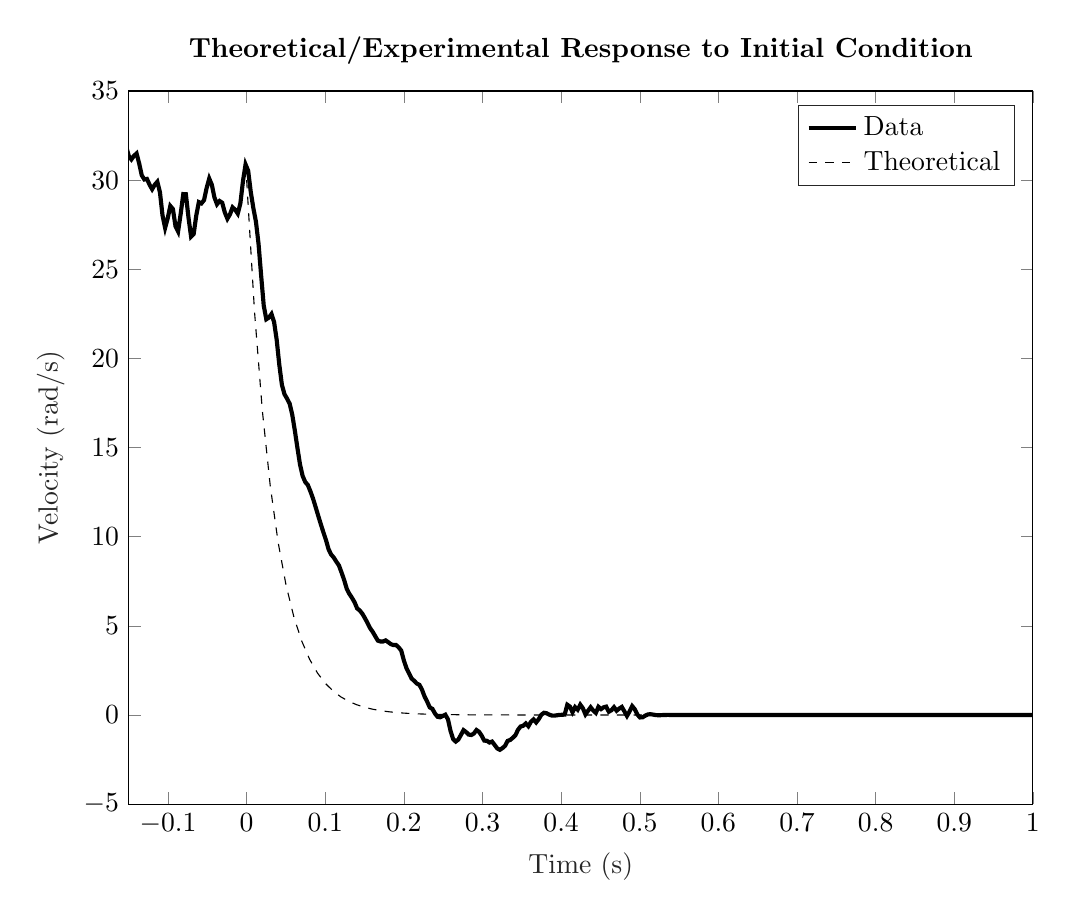
\begin{tikzpicture}

\begin{axis}[%
width=4.521in,
height=3.566in,
at={(0.758in,0.481in)},
scale only axis,
xmin=-0.15,
xmax=1,
xlabel style={font=\color{white!15!black}},
xlabel={Time (s)},
ymin=-5,
ymax=35,
ylabel style={font=\color{white!15!black}},
ylabel={Velocity (rad/s)},
axis background/.style={fill=white},
title style={font=\bfseries},
title={Theoretical/Experimental Response to Initial Condition},
legend style={legend cell align=left, align=left, draw=white!15!black}
]
\addplot [color=black, line width=1.5pt]
  table[row sep=crcr]{%
-0.800000011920929	31.9281539916992\\
-0.796700000762939	31.6026344299316\\
-0.79339998960495	31.8642559051514\\
-0.79009997844696	32.0763053894043\\
-0.786800026893616	31.4936256408691\\
-0.783500015735626	31.1619262695313\\
-0.780200004577637	31.3896961212158\\
-0.776899993419647	31.6282253265381\\
-0.773599982261658	31.1581115722656\\
-0.770299971103668	30.4812297821045\\
-0.767000019550323	30.0459632873535\\
-0.763700008392334	30.0001354217529\\
-0.760399997234344	29.7901248931885\\
-0.757099986076355	29.6040630340576\\
-0.753799974918365	29.6337604522705\\
-0.750500023365021	29.9035453796387\\
-0.747200012207031	29.5349388122559\\
-0.743900001049042	28.3903560638428\\
-0.740599989891052	27.4315204620361\\
-0.737299978733063	27.5776710510254\\
-0.734000027179718	28.5261573791504\\
-0.730700016021729	28.5484371185303\\
-0.727400004863739	27.6441993713379\\
-0.72409999370575	27.0182113647461\\
-0.72079998254776	27.7132320404053\\
-0.717500030994415	28.9378032684326\\
-0.714200019836426	29.3630275726318\\
-0.710900008678436	28.2664985656738\\
-0.707599997520447	26.9844875335693\\
-0.704299986362457	26.7912311553955\\
-0.700999975204468	27.7281398773193\\
-0.697700023651123	28.6694679260254\\
-0.694400012493134	28.7753486633301\\
-0.691100001335144	28.7654685974121\\
-0.687799990177155	29.2821998596191\\
-0.684499979019165	30.0268211364746\\
-0.68120002746582	29.9327964782715\\
-0.677900016307831	29.1903209686279\\
-0.674600005149841	28.655065536499\\
-0.671299993991852	28.697208404541\\
-0.667999982833862	28.7750301361084\\
-0.664700031280518	28.3268222808838\\
-0.661400020122528	27.9337120056152\\
-0.658100008964539	28.001501083374\\
-0.654799997806549	28.4477291107178\\
-0.65149998664856	28.3428688049316\\
-0.64819997549057	28.0315628051758\\
-0.644900023937225	28.4164028167725\\
-0.641600012779236	29.6298770904541\\
-0.638300001621246	30.7031154632568\\
-0.634999990463257	30.8011856079102\\
-0.631699979305267	29.8607559204102\\
-0.628400027751923	29.6174297332764\\
-0.625100016593933	30.2240924835205\\
-0.621800005435944	30.8713703155518\\
-0.618499994277954	30.2973937988281\\
-0.615199983119965	29.4487762451172\\
-0.61190003156662	29.5730876922607\\
-0.60860002040863	30.9739284515381\\
-0.605300009250641	32.4214172363281\\
-0.601999998092651	32.4837303161621\\
-0.598699986934662	32.163818359375\\
-0.595399975776672	32.2406845092773\\
-0.592100024223328	32.4417343139648\\
-0.588800013065338	31.985689163208\\
-0.585500001907349	31.7374114990234\\
-0.582199990749359	31.8526420593262\\
-0.57889997959137	32.0270538330078\\
-0.575600028038025	31.7280769348145\\
-0.572300016880035	31.164478302002\\
-0.569000005722046	31.2025737762451\\
-0.565699994564056	31.438081741333\\
-0.562399983406067	31.2450523376465\\
-0.559100031852722	30.5968132019043\\
-0.555800020694733	30.1329936981201\\
-0.552500009536743	29.9673156738281\\
-0.549199998378754	29.8577766418457\\
-0.545899987220764	29.5981464385986\\
-0.542599976062775	29.6474285125732\\
-0.53930002450943	29.919677734375\\
-0.53600001335144	29.7528591156006\\
-0.532700002193451	28.628885269165\\
-0.529399991035461	27.5998554229736\\
-0.526099979877472	27.439380645752\\
-0.522800028324127	28.3043079376221\\
-0.519500017166138	28.64723777771\\
-0.516200006008148	27.9121360778809\\
-0.512899994850159	27.0835990905762\\
-0.509599983692169	27.4338245391846\\
-0.50629997253418	28.7370586395264\\
-0.503000020980835	29.4783668518066\\
-0.499700009822845	28.6431198120117\\
-0.496399998664856	27.2302227020264\\
-0.493100017309189	26.6883735656738\\
-0.489800006151199	27.4956493377686\\
-0.486500024795532	28.5152606964111\\
-0.483200013637543	28.6828212738037\\
-0.479900002479553	28.5810775756836\\
-0.476600021123886	29.1324424743652\\
-0.473300009965897	29.9015789031982\\
-0.470000028610229	30.1449279785156\\
-0.46670001745224	29.5102424621582\\
-0.46340000629425	28.7667007446289\\
-0.460100024938583	28.561107635498\\
-0.456800013780594	28.7471179962158\\
-0.453500002622604	28.5444068908691\\
-0.450200021266937	28.1053123474121\\
-0.446900010108948	28.0180988311768\\
-0.443599998950958	28.2803401947021\\
-0.440300017595291	28.4086570739746\\
-0.437000006437302	28.0505180358887\\
-0.433700025081635	28.1298789978027\\
-0.430400013923645	29.1957206726074\\
-0.427100002765656	30.5517902374268\\
-0.423800021409988	30.8825969696045\\
-0.420500010251999	30.1633701324463\\
-0.417200028896332	29.5666999816895\\
-0.413900017738342	30.1507186889648\\
-0.410600006580353	30.8146858215332\\
-0.407300025224686	30.3911094665527\\
-0.404000014066696	29.4653911590576\\
-0.400700002908707	29.4191207885742\\
-0.39740002155304	30.6894836425781\\
-0.39410001039505	32.0690155029297\\
-0.390799999237061	32.461555480957\\
-0.387500017881393	32.4065856933594\\
-0.384200006723404	32.3511352539063\\
-0.380900025367737	32.3654632568359\\
-0.377600014209747	32.0267639160156\\
-0.374300003051758	31.6938438415527\\
-0.371000021696091	31.7559013366699\\
-0.367700010538101	31.9945106506348\\
-0.364400029182434	31.6760959625244\\
-0.361100018024445	31.2766704559326\\
-0.357800006866455	31.1562061309814\\
-0.354500025510788	31.4198131561279\\
-0.351200014352798	31.412317276001\\
-0.347900003194809	30.8455047607422\\
-0.344600021839142	30.2746906280518\\
-0.341300010681152	30.0209980010986\\
-0.337999999523163	29.9092845916748\\
-0.334700018167496	29.6342220306396\\
-0.331400007009506	29.547607421875\\
-0.328100025653839	29.9083003997803\\
-0.32480001449585	29.8398933410645\\
-0.32150000333786	29.030574798584\\
-0.318200021982193	27.7700977325439\\
-0.314900010824203	27.2930641174316\\
-0.311600029468536	28.0387668609619\\
-0.308300018310547	28.6056385040283\\
-0.305000007152557	28.0948543548584\\
-0.30170002579689	27.2379455566406\\
-0.298399984836578	27.1533164978027\\
-0.295100033283234	28.340404510498\\
-0.291800022125244	29.3354263305664\\
-0.288500010967255	28.9227275848389\\
-0.285199999809265	27.5598335266113\\
-0.281899988651276	26.7863082885742\\
-0.278600037097931	27.2406711578369\\
-0.275300025939941	28.2964973449707\\
-0.272000014781952	28.7351989746094\\
-0.268700003623962	28.6694469451904\\
-0.265399992465973	29.046070098877\\
-0.262100040912628	29.7987766265869\\
-0.258800029754639	30.1457042694092\\
-0.255500018596649	29.594633102417\\
-0.25220000743866	28.7419757843018\\
-0.248899981379509	28.5982513427734\\
-0.245600029826164	28.8129920959473\\
-0.242300018668175	28.7699413299561\\
-0.239000007510185	28.14453125\\
-0.235699996352196	27.8577423095703\\
-0.232399985194206	28.1934280395508\\
-0.229099974036217	28.478588104248\\
-0.225800022482872	28.1755485534668\\
-0.222500011324883	28.1316757202148\\
-0.219200000166893	28.8695850372314\\
-0.215899989008904	30.2926292419434\\
-0.212599977850914	30.8810558319092\\
-0.209300026297569	30.315113067627\\
-0.20600001513958	29.6775321960449\\
-0.20270000398159	29.8934917449951\\
-0.199399992823601	30.6374645233154\\
-0.196099981665611	30.636381149292\\
-0.192799970507622	29.7298622131348\\
-0.189500018954277	29.3248310089111\\
-0.186200007796288	30.2287006378174\\
-0.182899996638298	31.9649200439453\\
-0.179599985480309	32.4593696594238\\
-0.176299974322319	32.3121452331543\\
-0.173000022768974	32.3205261230469\\
-0.169700011610985	32.4208183288574\\
-0.166400000452995	32.1013984680176\\
-0.163099989295006	31.6667060852051\\
-0.159799978137016	31.6385860443115\\
-0.156500026583672	32.0014266967773\\
-0.153200015425682	31.877197265625\\
-0.149900004267693	31.3497409820557\\
-0.146599993109703	31.1603317260742\\
-0.143299981951714	31.361644744873\\
-0.140000030398369	31.4936103820801\\
-0.136700019240379	30.9320068359375\\
-0.13340000808239	30.266185760498\\
-0.1300999969244	30.0347785949707\\
-0.126799985766411	30.0636501312256\\
-0.123499974608421	29.743953704834\\
-0.120200023055077	29.4888439178467\\
-0.116900011897087	29.7380752563477\\
-0.113600000739098	29.9055843353271\\
-0.110299989581108	29.321756362915\\
-0.106999978423119	28.0160179138184\\
-0.103700026869774	27.3226337432861\\
-0.100400015711784	27.8621425628662\\
-0.0971000045537949	28.5487232208252\\
-0.0937999933958054	28.3755302429199\\
-0.0904999822378159	27.4142436981201\\
-0.0871999710798264	27.1242904663086\\
-0.0839000195264816	28.1123752593994\\
-0.0806000083684921	29.2147960662842\\
-0.0772999972105026	29.2058944702148\\
-0.0739999860525131	27.9057674407959\\
-0.0706999748945236	26.8273830413818\\
-0.0674000233411789	26.9754981994629\\
-0.0641000121831894	28.0117416381836\\
-0.0608000047504902	28.7648658752441\\
-0.0574999935925007	28.6958847045898\\
-0.0541999824345112	28.8791198730469\\
-0.0509000308811665	29.556001663208\\
-0.047600019723177	30.0847320556641\\
-0.0443000085651875	29.7381076812744\\
-0.040999997407198	29.0304756164551\\
-0.0376999862492085	28.6443862915039\\
-0.0344000346958637	28.8258800506592\\
-0.0311000235378742	28.7293109893799\\
-0.0278000123798847	28.1876430511475\\
-0.0245000012218952	27.8335380554199\\
-0.0211999900639057	28.0819091796875\\
-0.0178999789059162	28.4706325531006\\
-0.0146000264212489	28.3373889923096\\
-0.0113000152632594	28.1224403381348\\
-0.00800000410526991	28.6901302337646\\
-0.00469999294728041	29.9360103607178\\
-0.00139998202212155	30.8777446746826\\
0.00189996953122318	30.52903175354\\
0.00519998092204332	29.3440189361572\\
0.00849999208003283	28.4323806762695\\
0.0118000032380223	27.6697998046875\\
0.0151000143960118	26.4319801330566\\
0.0184000246226788	24.6613807678223\\
0.0216999761760235	22.9659786224365\\
0.024999987334013	22.1950397491455\\
0.0282999984920025	22.2865943908691\\
0.031600009649992	22.4888896942139\\
0.0349000208079815	22.0347213745117\\
0.0381999723613262	21.0387382507324\\
0.0414999835193157	19.6505088806152\\
0.0447999946773052	18.5228424072266\\
0.0481000058352947	17.9918518066406\\
0.0514000169932842	17.7423706054688\\
0.054699968546629	17.4592380523682\\
0.0579999797046185	16.8406352996826\\
0.061299990862608	15.9438104629517\\
0.0646000057458878	14.9710683822632\\
0.0679000169038773	14.0400362014771\\
0.071199968457222	13.4061040878296\\
0.0744999796152115	13.0657939910889\\
0.077799990773201	12.9007339477539\\
0.0811000019311905	12.5422115325928\\
0.08440001308918	12.1379766464233\\
0.0877000242471695	11.6656703948975\\
0.0909999758005142	11.1751947402954\\
0.0942999869585037	10.7027454376221\\
0.0975999981164932	10.2429990768433\\
0.100900009274483	9.80929946899414\\
0.104200020432472	9.29401588439941\\
0.107499971985817	8.99793910980225\\
0.110799983143806	8.82920742034912\\
0.114099994301796	8.59646701812744\\
0.117400005459785	8.38499927520752\\
0.120700016617775	7.98673963546753\\
0.124000027775764	7.56928873062134\\
0.127299979329109	7.08126258850098\\
0.130599990487099	6.79544878005981\\
0.133900001645088	6.57446002960205\\
0.137200012803078	6.3285174369812\\
0.140500023961067	5.97795486450195\\
0.143799975514412	5.86473989486694\\
0.147099986672401	5.68036890029907\\
0.150399997830391	5.43462705612183\\
0.15370000898838	5.16075563430786\\
0.15700002014637	4.86994600296021\\
0.160299971699715	4.6645040512085\\
0.163599982857704	4.41404151916504\\
0.166899994015694	4.17146968841553\\
0.170200005173683	4.12332057952881\\
0.173500016331673	4.12392282485962\\
0.176799967885017	4.18353080749512\\
0.180099979043007	4.08205795288086\\
0.183399990200996	3.97324132919312\\
0.186700001358986	3.92066693305969\\
0.190000012516975	3.92529082298279\\
0.193300023674965	3.79481029510498\\
0.19659997522831	3.61047172546387\\
0.199899986386299	3.06437158584595\\
0.203200057148933	2.63098478317261\\
0.206500008702278	2.3369140625\\
0.209799960255623	2.04019832611084\\
0.213100031018257	1.91843557357788\\
0.216399982571602	1.76182699203491\\
0.219700053334236	1.69399416446686\\
0.223000004887581	1.41884982585907\\
0.226299956440926	1.03294599056244\\
0.22960002720356	0.746708512306213\\
0.232899978756905	0.424585193395615\\
0.236200049519539	0.346733510494232\\
0.239500001072884	0.082810714840889\\
0.242799952626228	-0.102074079215527\\
0.246100023388863	-0.127591028809547\\
0.249399974942207	-0.0573741532862186\\
0.25270003080368	0.0147751802578568\\
0.255999982357025	-0.242807954549789\\
0.25929993391037	-0.892208993434906\\
0.262600004673004	-1.3497759103775\\
0.265899956226349	-1.48955166339874\\
0.269200026988983	-1.37811744213104\\
0.272499978542328	-1.11974120140076\\
0.275799930095673	-0.850398361682892\\
0.279100000858307	-0.95745176076889\\
0.282399952411652	-1.09788000583649\\
0.285700023174286	-1.12363624572754\\
0.288999974727631	-1.0392017364502\\
0.292299926280975	-0.843660414218903\\
0.29559999704361	-0.944307625293732\\
0.298899948596954	-1.15920615196228\\
0.302200019359589	-1.43805313110352\\
0.305499970912933	-1.44801497459412\\
0.308799922466278	-1.54468476772308\\
0.312099993228912	-1.49008166790009\\
0.315399944782257	-1.68151557445526\\
0.318700015544891	-1.87494039535522\\
0.321999967098236	-1.95245027542114\\
0.32530003786087	-1.85825765132904\\
0.328599989414215	-1.7286479473114\\
0.33189994096756	-1.45344376564026\\
0.335200011730194	-1.40045857429504\\
0.338499963283539	-1.27725780010223\\
0.341800034046173	-1.13697791099548\\
0.345099985599518	-0.830001950263977\\
0.348399937152863	-0.644509732723236\\
0.351700007915497	-0.605646908283234\\
0.354999959468842	-0.47559055685997\\
0.358300030231476	-0.628804385662079\\
0.361599981784821	-0.37827867269516\\
0.364899933338165	-0.248897165060043\\
0.3682000041008	-0.417771130800247\\
0.371499955654144	-0.230239585042\\
0.374800026416779	0.0124823348596692\\
0.378099977970123	0.124930016696453\\
0.381399929523468	0.0996201932430267\\
0.384700000286102	0.0223310459405184\\
0.387999951839447	-0.0305642113089561\\
0.391300022602081	-0.0369803085923195\\
0.394599974155426	-0.0161424428224564\\
0.397899925708771	0.00469428393989801\\
0.401199996471405	0.0119938896968961\\
0.40449994802475	0.0218656118959188\\
0.407800018787384	0.573133766651154\\
0.411099970340729	0.474596858024597\\
0.414400041103363	0.159132793545723\\
0.417699992656708	0.441458463668823\\
0.420999944210052	0.294891506433487\\
0.424300014972687	0.578290462493896\\
0.427599966526031	0.379236072301865\\
0.430900037288666	0.0339901447296143\\
0.434199988842011	0.236483201384544\\
0.437499940395355	0.432906985282898\\
0.44080001115799	0.249226540327072\\
0.444099962711334	0.116379097104073\\
0.447400033473969	0.45788249373436\\
0.450699985027313	0.330035030841827\\
0.453999936580658	0.431234985589981\\
0.457300007343292	0.468605816364288\\
0.460599958896637	0.182731673121452\\
0.463900029659271	0.265137672424316\\
0.467199981212616	0.437051028013229\\
0.470499932765961	0.238511130213737\\
0.473800003528595	0.360767841339111\\
0.47709995508194	0.452056735754013\\
0.480400025844574	0.203715920448303\\
0.483699977397919	-0.0519773438572884\\
0.486999928951263	0.197900652885437\\
0.490299999713898	0.496674418449402\\
0.493599951267242	0.322405934333801\\
0.496900022029877	0.0263952985405922\\
0.500199973583221	-0.137776330113411\\
0.503499925136566	-0.129810601472855\\
0.5067999958992	-0.0415211506187916\\
0.510099947452545	0.0293057151138783\\
0.513400018215179	0.0454455502331257\\
0.516699969768524	0.023937763646245\\
0.519999921321869	-0.00229634763672948\\
0.523299992084503	-0.0138345966115594\\
0.526599943637848	-0.0105777634307742\\
0.529900014400482	-0.00208821659907699\\
0.533199965953827	0.00348505889996886\\
0.536500036716461	0.00398915586993098\\
0.539799988269806	0.00164794293232262\\
0.543099939823151	-0.000585504225455225\\
0.546400010585785	-0.00131445331498981\\
0.54969996213913	-0.000822567730210721\\
0.553000032901764	-4.38681890955195e-05\\
0.556299984455109	0.000371398782590404\\
0.559599936008453	0.000336375524057075\\
0.562900006771088	0.000100451230537146\\
0.566199958324432	-8.19873748696409e-05\\
0.569500029087067	-0.000119338350486942\\
0.572799980640411	-6.03616281296127e-05\\
0.576099932193756	8.14549275673926e-06\\
0.57940000295639	3.68803885066882e-05\\
0.582699954509735	2.71930639428319e-05\\
0.586000025272369	4.71527346235234e-06\\
0.589299976825714	-9.5124778454192e-06\\
0.592599928379059	-1.03992597360048e-05\\
0.595899999141693	-4.08376672567101e-06\\
0.599199950695038	1.70608666394401e-06\\
0.602500021457672	3.4734557630145e-06\\
0.605799973011017	2.09471704692987e-06\\
0.609099924564362	4.90576610445714e-08\\
0.612399995326996	-9.98864607026917e-07\\
0.615699946880341	-8.70432188548875e-07\\
0.619000017642975	-2.41147830593036e-07\\
0.62229996919632	2.28073020025477e-07\\
0.625600039958954	3.12959798520751e-07\\
0.628899991512299	1.51805139125827e-07\\
0.632199943065643	-2.68597037944573e-08\\
0.635500013828278	-9.81506147468281e-08\\
0.638799965381622	-6.97947655226017e-08\\
0.642100036144257	-1.03674846485546e-08\\
0.645399987697601	2.58845620493275e-08\\
0.648699939250946	2.70742503971633e-08\\
0.65200001001358	1.00760697563373e-08\\
0.655299961566925	-4.91263429935884e-09\\
0.658600032329559	-9.1658707290776e-09\\
0.661899983882904	-5.32374722084228e-09\\
0.665199935436249	4.32169716679809e-11\\
0.668500006198883	2.68082755994214e-09\\
0.671799957752228	2.24926632874656e-09\\
0.675100028514862	5.73669778347607e-10\\
0.678399980068207	-6.3125821236909e-10\\
0.681699931621552	-8.19627754555796e-10\\
0.685000002384186	-3.80712961156604e-10\\
0.688299953937531	8.46245296060033e-11\\
0.691600024700165	2.60774651872353e-10\\
0.69489997625351	1.78850101395511e-10\\
0.698199927806854	2.19680766633257e-11\\
0.701499998569489	-7.02246663597528e-11\\
0.704799950122833	-7.03940863933106e-11\\
0.708100020885468	-2.47473343900628e-11\\
0.711399972438812	1.40020208969083e-11\\
0.714699923992157	2.41516737164993e-11\\
0.717999994754791	1.35024231379122e-11\\
0.721299946308136	-5.58860087113838e-13\\
0.72460001707077	-7.17986347459343e-12\\
0.727899968624115	-5.80391203847119e-12\\
0.73119992017746	-1.3499017442048e-12\\
0.734499990940094	1.73932417947553e-12\\
0.737799942493439	2.14374937072825e-12\\
0.741100013256073	9.51912593888382e-13\\
0.744399964809418	-2.58476400005758e-13\\
0.747700035572052	-6.91740393264639e-13\\
0.750999987125397	-4.5754367091963e-13\\
0.754299938678741	-4.39776931234273e-14\\
0.757600009441376	1.90004953502625e-13\\
0.76089996099472	1.82783828220692e-13\\
0.764200031757355	6.04508983018462e-14\\
0.767499983310699	-3.95823951144115e-14\\
0.770799934864044	-6.35524212465668e-14\\
0.774100005626678	-3.41710200987919e-14\\
0.777399957180023	2.62155892493906e-15\\
0.780700027942657	1.91927281223891e-14\\
0.783999979496002	1.49546309580542e-14\\
0.787299931049347	3.13398971758892e-15\\
0.790600001811981	-4.77320175843333e-15\\
0.793899953365326	-5.59963740550925e-15\\
0.79720002412796	-2.37230529240762e-15\\
0.800499975681305	7.71848397031877e-16\\
0.80379992723465	1.83205857304464e-15\\
0.807099997997284	1.16843832854052e-15\\
0.810399949550629	7.97405419223569e-17\\
0.813700020313263	-5.12804969454305e-16\\
0.816999971866608	-4.73962791350301e-16\\
0.820299923419952	-1.46754096174863e-16\\
0.823599994182587	1.11105708738041e-16\\
0.826899945735931	1.67000420310617e-16\\
0.830200016498566	8.62692336517766e-17\\
0.83349996805191	-9.87407317001897e-18\\
0.836800038814545	-5.12123862320483e-17\\
0.840099990367889	-3.84742316239278e-17\\
0.843399941921234	-7.15201037128662e-18\\
0.846700012683868	1.30517288521721e-17\\
0.849999964237213	1.46073776516985e-17\\
0.853300034999847	5.89011367320278e-18\\
0.856599986553192	-2.26618743313243e-18\\
0.859899938106537	-4.84503714369103e-18\\
0.863200008869171	-2.97833059033164e-18\\
0.866499960422516	-1.16301542426167e-19\\
0.86980003118515	1.38078964227277e-18\\
0.873099982738495	1.22733647170591e-18\\
0.87639993429184	3.53779952260707e-19\\
0.879700005054474	-3.09936329566888e-19\\
0.882999956607819	-4.38241736096666e-19\\
0.886300027370453	-2.17260047712213e-19\\
0.889599978923798	3.36437393397846e-20\\
0.892899930477142	1.3640726581352e-19\\
0.896200001239777	9.88305056120701e-20\\
0.899499952793121	1.59608295821871e-20\\
0.902800023555756	-3.55683915235651e-20\\
0.9060999751091	-3.8054660569178e-20\\
0.909399926662445	-1.45670544838423e-20\\
0.912699997425079	6.5624947430327e-21\\
0.915999948978424	1.27938425912314e-20\\
0.919300019741058	7.57720543994588e-21\\
0.922599971294403	6.35314494273897e-23\\
0.925899922847748	-3.7096808845855e-21\\
0.929199993610382	-3.17379063227332e-21\\
0.932499945163727	-8.45762489921886e-22\\
0.935800015926361	8.59997125236026e-22\\
0.939099967479706	1.14851655159385e-21\\
0.942399919033051	5.45676519914447e-22\\
0.945699989795685	-1.08247076895869e-22\\
0.94899994134903	-3.62717385939956e-22\\
0.952300012111664	-2.5346593133956e-22\\
0.955599963665009	-3.45356236112048e-23\\
0.958900034427643	9.6640029971937e-23\\
0.962199985980988	9.90111439046396e-23\\
0.965499937534332	3.58668484768706e-23\\
0.968800008296967	-1.87972111524342e-23\\
0.972099959850311	-3.37364191617945e-23\\
0.975400030612946	-1.92394039774122e-23\\
0.97869998216629	4.6004760688395e-25\\
0.981999933719635	9.94564274866443e-24\\
0.985300004482269	8.19572522438714e-24\\
0.988599956035614	2.002169998218e-24\\
0.991900026798248	-2.37481625414605e-24\\
0.995199978351593	-3.00599766947923e-24\\
0.998499929904938	-1.36661996979933e-24\\
1.00180006027222	3.3547865529621e-25\\
1.00510001182556	9.62940911936009e-25\\
1.0084000825882	6.49011446728205e-25\\
1.01170003414154	7.14567834060044e-26\\
1.01499998569489	-2.61828776943933e-25\\
1.01830005645752	-2.57267903664688e-25\\
1.02160000801086	-8.78682395152465e-26\\
1.0249000787735	5.33550387329307e-26\\
1.02820003032684	8.88365601134294e-26\\
1.03149998188019	4.87468615327635e-26\\
1.03480005264282	-2.83417674315188e-27\\
1.03810000419617	-2.66125338679098e-26\\
1.0414000749588	-2.11338409551115e-26\\
1.04470002651215	-4.68288248196603e-27\\
1.04800009727478	6.53031614405191e-27\\
1.05130004882813	7.85728341647867e-27\\
1.05460000038147	3.41186501516767e-27\\
1.0579000711441	-1.01262237950772e-27\\
1.06120002269745	-2.55235811069162e-27\\
1.06450009346008	-1.65897140219188e-27\\
1.06780004501343	-1.37473553505841e-28\\
1.07109999656677	7.07545061481072e-28\\
1.07440006732941	6.67590874412781e-28\\
1.07770001888275	2.14042028081116e-28\\
1.08100008964539	-1.50282997825396e-28\\
1.08430004119873	-2.33604228156991e-28\\
1.08759999275208	-1.2322622192687e-28\\
1.09090006351471	1.16525156324696e-29\\
1.09420001506805	7.10746570938813e-29\\
1.09750008583069	5.44149839074739e-29\\
1.10080003738403	1.07898314250678e-29\\
1.10409998893738	-1.78877755173668e-29\\
1.10740005970001	-2.05105279804921e-29\\
1.11070001125336	-8.48853999146866e-30\\
1.11400008201599	2.99716452905995e-30\\
1.11730003356934	6.75483440649173e-30\\
1.12059998512268	4.2328754117743e-30\\
1.12390005588531	2.30309671080337e-31\\
1.12720000743866	-1.90733136680807e-30\\
1.13050007820129	-1.72994682424074e-30\\
1.13380002975464	-5.17979328740687e-31\\
1.13709998130798	4.20497086859764e-31\\
1.14040005207062	6.13442917682831e-31\\
1.14370000362396	3.10747832621513e-31\\
1.1470000743866	-4.14733743852174e-32\\
1.15030002593994	-1.89473032597602e-31\\
1.15359997749329	-1.39888800088956e-31\\
1.15690004825592	-2.43814866902217e-32\\
1.16019999980927	4.88288480838635e-32\\
1.1635000705719	5.34696174963053e-32\\
1.16680002212524	2.10381574125565e-32\\
1.17010009288788	-8.73772868957038e-33\\
1.17340004444122	-1.78506017075263e-32\\
1.17669999599457	-1.07802066947897e-32\\
1.1800000667572	-2.64910049749784e-34\\
1.18330001831055	5.1300046511243e-33\\
1.18660008907318	4.47685848016317e-33\\
1.18990004062653	1.24404954870423e-33\\
1.19319999217987	-1.16984362090819e-33\\
1.1965000629425	-1.60878469094225e-33\\
1.19980001449585	-7.8163302996478e-34\\
1.20309996604919	1.36998505691249e-34\\
1.20640015602112	5.04270454277957e-34\\
1.20970010757446	3.59087259224308e-34\\
1.21300005912781	5.36959103984964e-35\\
1.21630001068115	-1.32871958027449e-34\\
1.2195999622345	-1.3921681505982e-34\\
1.22290015220642	-5.19246734443788e-35\\
1.22620010375977	2.51656494437225e-35\\
1.22950005531311	4.71062601113983e-35\\
1.23280000686646	2.74010746528893e-35\\
1.2360999584198	-1.87348806634286e-37\\
1.23940014839172	-1.37684238471202e-35\\
1.24270009994507	-1.15692069347082e-35\\
1.24600005149841	-2.96090338740567e-36\\
1.24930000305176	3.23827671932498e-36\\
1.2525999546051	4.21355282809972e-36\\
1.25590014457703	1.96057538036356e-36\\
1.25920009613037	-4.3215345111584e-37\\
1.26250004768372	-1.33983056323915e-36\\
1.26579999923706	-9.20232746363658e-37\\
1.26909995079041	-1.13984599051313e-37\\
1.27240014076233	3.60521091489344e-37\\
1.27570009231567	3.61990638794075e-37\\
1.27900004386902	1.27550513432503e-37\\
1.28229999542236	-7.17572937923814e-38\\
1.28559994697571	-1.2413355362593e-37\\
1.28890013694763	-6.95038601267068e-38\\
1.29220008850098	2.7833669098237e-39\\
1.29550004005432	3.68793281425497e-38\\
1.29879999160767	2.98557764134209e-38\\
1.30209994316101	6.97135476263114e-39\\
1.30540013313293	-8.92396187787988e-39\\
1.30870008468628	-1.1021415610192e-38\\
1.31200003623962	-4.90302421630307e-39\\
1.31529998779297	1.32124088175948e-39\\
1.31859993934631	3.55440616644608e-39\\
1.32190012931824	2.35450091611556e-39\\
1.32520008087158	2.2888949246128e-40\\
1.32850003242493	-9.75582589564473e-40\\
1.33179998397827	-9.40051265703053e-40\\
1.33509993553162	-3.11665594047411e-40\\
1.33840012550354	2.02968273468199e-40\\
1.34170007705688	3.26770190194368e-40\\
1.34500002861023	1.76075954639342e-40\\
1.34829998016357	-1.31525873861527e-41\\
1.35159993171692	-9.86710300669677e-41\\
1.35490012168884	-7.70433895685784e-41\\
1.35820007324219	-1.62046154414522e-41\\
1.36150002479553	2.45283283195416e-41\\
1.36479997634888	2.88387223958047e-41\\
1.36809992790222	1.21716784611254e-41\\
1.37140011787415	-4.06656814347062e-42\\
1.37470006942749	-9.30742440004544e-42\\
1.37800002098084	-5.81258603001934e-42\\
1.38129997253418	-2.85864886722263e-43\\
1.38459992408752	2.6708748730031e-42\\
1.38790011405945	2.40602946324571e-42\\
1.39120006561279	7.83325841557573e-43\\
1.39450001716614	-5.24085625657482e-43\\
1.39779996871948	-8.63199854024087e-43\\
1.40109992027283	-4.07777853118522e-43\\
1.40440011024475	9.66895940384124e-44\\
1.4077000617981	2.95673975972536e-43\\
1.41100001335144	1.33123354110858e-43\\
1.41429996490479	-6.30584308946168e-44\\
1.41759991645813	-1.00893489431387e-43\\
1.42090010643005	-1.00893489431387e-43\\
1.4242000579834	-1.00893489431387e-43\\
1.42750000953674	-1.00893489431387e-43\\
1.43079996109009	-1.00893489431387e-43\\
1.43410015106201	-1.00893489431387e-43\\
1.43740010261536	-1.00893489431387e-43\\
1.4407000541687	-1.00893489431387e-43\\
1.44400000572205	-1.00893489431387e-43\\
1.44729995727539	-1.00893489431387e-43\\
1.45060014724731	-1.00893489431387e-43\\
1.45390009880066	-1.00893489431387e-43\\
1.457200050354	-1.00893489431387e-43\\
1.46050000190735	-1.00893489431387e-43\\
1.46379995346069	-1.00893489431387e-43\\
1.46710014343262	-1.00893489431387e-43\\
1.47040009498596	-1.00893489431387e-43\\
1.47370004653931	-1.00893489431387e-43\\
1.47699999809265	-1.00893489431387e-43\\
1.480299949646	-1.00893489431387e-43\\
1.48360013961792	-1.00893489431387e-43\\
1.48690009117126	-1.00893489431387e-43\\
1.49020004272461	-1.00893489431387e-43\\
1.49349999427795	-1.00893489431387e-43\\
1.4967999458313	-1.00893489431387e-43\\
1.50010013580322	-1.00893489431387e-43\\
1.50340008735657	-1.00893489431387e-43\\
1.50670003890991	-1.00893489431387e-43\\
1.50999999046326	-1.00893489431387e-43\\
1.5132999420166	-1.00893489431387e-43\\
1.51660013198853	-1.00893489431387e-43\\
1.51990008354187	-1.00893489431387e-43\\
1.52320003509521	-1.00893489431387e-43\\
1.52649998664856	-1.00893489431387e-43\\
1.5297999382019	-1.00893489431387e-43\\
1.53310012817383	-1.00893489431387e-43\\
1.53640007972717	-1.00893489431387e-43\\
1.53970003128052	-1.00893489431387e-43\\
1.54299998283386	-1.00893489431387e-43\\
1.54629993438721	-1.00893489431387e-43\\
1.54960012435913	-1.00893489431387e-43\\
1.55290007591248	-1.00893489431387e-43\\
1.55620002746582	-1.00893489431387e-43\\
1.55949997901917	-1.00893489431387e-43\\
1.56279993057251	-1.00893489431387e-43\\
1.56610012054443	-1.00893489431387e-43\\
1.56940007209778	-1.00893489431387e-43\\
1.57270002365112	-1.00893489431387e-43\\
1.57599997520447	-1.00893489431387e-43\\
1.57929992675781	-1.00893489431387e-43\\
1.58260011672974	-1.00893489431387e-43\\
1.58590006828308	-1.00893489431387e-43\\
1.58920001983643	-1.00893489431387e-43\\
1.59249997138977	-1.00893489431387e-43\\
1.59579992294312	-1.00893489431387e-43\\
1.59910011291504	-1.00893489431387e-43\\
1.60240006446838	-1.00893489431387e-43\\
1.60570001602173	-1.00893489431387e-43\\
1.60899996757507	-1.00893489431387e-43\\
1.61229991912842	-1.00893489431387e-43\\
1.61560010910034	-1.00893489431387e-43\\
1.61890006065369	-1.00893489431387e-43\\
1.62220001220703	-1.00893489431387e-43\\
1.62549996376038	-1.00893489431387e-43\\
1.6288001537323	-1.00893489431387e-43\\
1.63210010528564	-1.00893489431387e-43\\
1.63540005683899	-1.00893489431387e-43\\
1.63870000839233	-1.00893489431387e-43\\
1.64199995994568	-1.00893489431387e-43\\
1.6453001499176	-1.00893489431387e-43\\
1.64860010147095	-1.00893489431387e-43\\
1.65190005302429	-1.00893489431387e-43\\
1.65520000457764	-1.00893489431387e-43\\
1.65849995613098	-1.00893489431387e-43\\
1.66180014610291	-1.00893489431387e-43\\
1.66510009765625	-1.00893489431387e-43\\
1.66840004920959	-1.00893489431387e-43\\
1.67170000076294	-1.00893489431387e-43\\
1.67499995231628	-1.00893489431387e-43\\
1.67830014228821	-1.00893489431387e-43\\
1.68160009384155	-1.00893489431387e-43\\
1.6849000453949	-1.00893489431387e-43\\
1.68819999694824	-1.00893489431387e-43\\
1.69149994850159	-1.00893489431387e-43\\
1.69480013847351	-1.00893489431387e-43\\
1.69810009002686	-1.00893489431387e-43\\
1.7014000415802	-1.00893489431387e-43\\
1.70469999313354	-1.00893489431387e-43\\
1.70799994468689	-1.00893489431387e-43\\
1.71130013465881	-1.00893489431387e-43\\
1.71460008621216	-1.00893489431387e-43\\
1.7179000377655	-1.00893489431387e-43\\
1.72119998931885	-1.00893489431387e-43\\
1.72449994087219	-1.00893489431387e-43\\
1.72780013084412	-1.00893489431387e-43\\
1.73110008239746	-1.00893489431387e-43\\
1.73440003395081	-1.00893489431387e-43\\
1.73769998550415	-1.00893489431387e-43\\
1.7409999370575	-1.00893489431387e-43\\
1.74430012702942	-1.00893489431387e-43\\
1.74760007858276	-1.00893489431387e-43\\
1.75090003013611	-1.00893489431387e-43\\
1.75419998168945	-1.00893489431387e-43\\
1.7574999332428	-1.00893489431387e-43\\
1.76080012321472	-1.00893489431387e-43\\
1.76410007476807	-1.00893489431387e-43\\
1.76740002632141	-1.00893489431387e-43\\
1.77069997787476	-1.00893489431387e-43\\
1.7739999294281	-1.00893489431387e-43\\
1.77730011940002	-1.00893489431387e-43\\
1.78060007095337	-1.00893489431387e-43\\
1.78390002250671	-1.00893489431387e-43\\
1.78719997406006	-1.00893489431387e-43\\
1.7904999256134	-1.00893489431387e-43\\
1.79380011558533	-1.00893489431387e-43\\
1.79710006713867	-1.00893489431387e-43\\
1.80040001869202	-1.00893489431387e-43\\
1.80369997024536	-1.00893489431387e-43\\
1.80699992179871	-1.00893489431387e-43\\
1.81030011177063	-1.00893489431387e-43\\
1.81360006332397	-1.00893489431387e-43\\
1.81690001487732	-1.00893489431387e-43\\
1.82019996643066	-1.00893489431387e-43\\
1.82349991798401	-1.00893489431387e-43\\
1.82680010795593	-1.00893489431387e-43\\
1.83010005950928	-1.00893489431387e-43\\
1.83340001106262	-1.00893489431387e-43\\
1.83669996261597	-1.00893489431387e-43\\
1.83999991416931	-1.00893489431387e-43\\
1.84330010414124	-1.00893489431387e-43\\
1.84660005569458	-1.00893489431387e-43\\
1.84990000724792	-1.00893489431387e-43\\
1.85319995880127	-1.00893489431387e-43\\
1.85650014877319	-1.00893489431387e-43\\
1.85980010032654	-1.00893489431387e-43\\
1.86310005187988	-1.00893489431387e-43\\
1.86640000343323	-1.00893489431387e-43\\
1.86969995498657	-1.00893489431387e-43\\
1.8730001449585	-1.00893489431387e-43\\
1.87630009651184	-1.00893489431387e-43\\
1.87960004806519	-1.00893489431387e-43\\
1.88289999961853	-1.00893489431387e-43\\
1.88619995117188	-1.00893489431387e-43\\
1.8895001411438	-1.00893489431387e-43\\
1.89280009269714	-1.00893489431387e-43\\
1.89610004425049	-1.00893489431387e-43\\
1.89939999580383	-1.00893489431387e-43\\
1.90269994735718	-1.00893489431387e-43\\
1.9060001373291	-1.00893489431387e-43\\
1.90930008888245	-1.00893489431387e-43\\
1.91260004043579	-1.00893489431387e-43\\
1.91589999198914	-1.00893489431387e-43\\
1.91919994354248	-1.00893489431387e-43\\
1.9225001335144	-1.00893489431387e-43\\
1.92580008506775	-1.00893489431387e-43\\
1.92910003662109	-1.00893489431387e-43\\
1.93239998817444	-1.00893489431387e-43\\
1.93569993972778	-1.00893489431387e-43\\
1.93900012969971	-1.00893489431387e-43\\
1.94230008125305	-1.00893489431387e-43\\
1.9456000328064	-1.00893489431387e-43\\
1.94889998435974	-1.00893489431387e-43\\
1.95219993591309	-1.00893489431387e-43\\
1.95550012588501	-1.00893489431387e-43\\
1.95880007743835	-1.00893489431387e-43\\
1.9621000289917	-1.00893489431387e-43\\
1.96539998054504	-1.00893489431387e-43\\
1.96869993209839	-1.00893489431387e-43\\
1.97200012207031	-1.00893489431387e-43\\
1.97530007362366	-1.00893489431387e-43\\
1.978600025177	-1.00893489431387e-43\\
1.98189997673035	-1.00893489431387e-43\\
1.98519992828369	-1.00893489431387e-43\\
1.98850011825562	-1.00893489431387e-43\\
1.99180006980896	-1.00893489431387e-43\\
1.9951000213623	-1.00893489431387e-43\\
1.99839997291565	-1.00893489431387e-43\\
2.00169992446899	-1.00893489431387e-43\\
2.00500011444092	-1.00893489431387e-43\\
2.00830006599426	-1.00893489431387e-43\\
2.01160001754761	-1.00893489431387e-43\\
2.01489996910095	-1.00893489431387e-43\\
2.0181999206543	-1.00893489431387e-43\\
2.02150011062622	-1.00893489431387e-43\\
2.02480006217957	-1.00893489431387e-43\\
2.02810001373291	-1.00893489431387e-43\\
2.03139996528625	-1.00893489431387e-43\\
2.0346999168396	-1.00893489431387e-43\\
2.03800010681152	-1.00893489431387e-43\\
2.04130005836487	-1.00893489431387e-43\\
2.04460000991821	-1.00893489431387e-43\\
2.04789996147156	-1.00893489431387e-43\\
2.05120015144348	-1.00893489431387e-43\\
2.05450010299683	-1.00893489431387e-43\\
2.05780005455017	-1.00893489431387e-43\\
2.06110000610352	-1.00893489431387e-43\\
2.06439995765686	-1.00893489431387e-43\\
2.06770014762878	-1.00893489431387e-43\\
2.07100009918213	-1.00893489431387e-43\\
2.07430005073547	-1.00893489431387e-43\\
2.07760000228882	-1.00893489431387e-43\\
2.08089995384216	-1.00893489431387e-43\\
2.08420014381409	-1.00893489431387e-43\\
2.08750009536743	-1.00893489431387e-43\\
2.09080004692078	-1.00893489431387e-43\\
2.09409999847412	-1.00893489431387e-43\\
2.09739995002747	-1.00893489431387e-43\\
2.10070013999939	-1.00893489431387e-43\\
2.10400009155273	-1.00893489431387e-43\\
2.10730004310608	-1.00893489431387e-43\\
2.11059999465942	-1.00893489431387e-43\\
2.11389994621277	-1.00893489431387e-43\\
2.11720013618469	-1.00893489431387e-43\\
2.12050008773804	-1.00893489431387e-43\\
2.12380003929138	-1.00893489431387e-43\\
2.12709999084473	-1.00893489431387e-43\\
2.13039994239807	-1.00893489431387e-43\\
2.13370013237	-1.00893489431387e-43\\
2.13700008392334	-1.00893489431387e-43\\
2.14030003547668	-1.00893489431387e-43\\
2.14359998703003	-1.00893489431387e-43\\
2.14689993858337	-1.00893489431387e-43\\
2.1502001285553	-1.00893489431387e-43\\
2.15350008010864	-1.00893489431387e-43\\
2.15680003166199	-1.00893489431387e-43\\
2.16009998321533	-1.00893489431387e-43\\
2.16339993476868	-1.00893489431387e-43\\
2.1667001247406	-1.00893489431387e-43\\
2.17000007629395	-1.00893489431387e-43\\
2.17330002784729	-1.00893489431387e-43\\
2.17659997940063	-1.00893489431387e-43\\
2.17989993095398	-1.00893489431387e-43\\
2.1832001209259	-1.00893489431387e-43\\
2.18650007247925	-1.00893489431387e-43\\
2.18980002403259	-1.00893489431387e-43\\
2.19309997558594	-1.00893489431387e-43\\
2.19639992713928	-1.00893489431387e-43\\
2.19970011711121	-1.00893489431387e-43\\
2.20300006866455	-1.00893489431387e-43\\
2.2063000202179	-1.00893489431387e-43\\
2.20959997177124	-1.00893489431387e-43\\
2.21289992332459	-1.00893489431387e-43\\
2.21620011329651	-1.00893489431387e-43\\
2.21950006484985	-1.00893489431387e-43\\
2.2228000164032	-1.00893489431387e-43\\
2.22609996795654	-1.00893489431387e-43\\
2.22939991950989	-1.00893489431387e-43\\
2.23270010948181	-1.00893489431387e-43\\
2.23600006103516	-1.00893489431387e-43\\
2.2393000125885	-1.00893489431387e-43\\
2.24259996414185	-1.00893489431387e-43\\
2.24589991569519	-1.00893489431387e-43\\
2.24920010566711	-1.00893489431387e-43\\
2.25250005722046	-1.00893489431387e-43\\
2.2558000087738	-1.00893489431387e-43\\
2.25909996032715	-1.00893489431387e-43\\
2.26239991188049	-1.00893489431387e-43\\
2.26570010185242	-1.00893489431387e-43\\
2.26900005340576	-1.00893489431387e-43\\
2.27230000495911	-1.00893489431387e-43\\
2.27559995651245	-1.00893489431387e-43\\
2.27890014648438	-1.00893489431387e-43\\
2.28220009803772	-1.00893489431387e-43\\
2.28550004959106	-1.00893489431387e-43\\
2.28880000114441	-1.00893489431387e-43\\
2.29209995269775	-1.00893489431387e-43\\
2.29540014266968	-1.00893489431387e-43\\
2.29870009422302	-1.00893489431387e-43\\
2.30200004577637	-1.00893489431387e-43\\
2.30529999732971	-1.00893489431387e-43\\
2.30859994888306	-1.00893489431387e-43\\
2.31190013885498	-1.00893489431387e-43\\
2.31520009040833	-1.00893489431387e-43\\
2.31850004196167	-1.00893489431387e-43\\
2.32179999351501	-1.00893489431387e-43\\
2.32509994506836	-1.00893489431387e-43\\
2.32840013504028	-1.00893489431387e-43\\
2.33170008659363	-1.00893489431387e-43\\
2.33500003814697	-1.00893489431387e-43\\
2.33829998970032	-1.00893489431387e-43\\
2.34159994125366	-1.00893489431387e-43\\
2.34490013122559	-1.00893489431387e-43\\
2.34820008277893	-1.00893489431387e-43\\
2.35150003433228	-1.00893489431387e-43\\
2.35479998588562	-1.00893489431387e-43\\
2.35809993743896	-1.00893489431387e-43\\
2.36140012741089	-1.00893489431387e-43\\
2.36470007896423	-1.00893489431387e-43\\
2.36800003051758	-1.00893489431387e-43\\
2.37129998207092	-1.00893489431387e-43\\
2.37459993362427	-1.00893489431387e-43\\
2.37790012359619	-1.00893489431387e-43\\
2.38120007514954	-1.00893489431387e-43\\
2.38450002670288	-1.00893489431387e-43\\
2.38779997825623	-1.00893489431387e-43\\
2.39109992980957	-1.00893489431387e-43\\
2.39440011978149	-1.00893489431387e-43\\
2.39770007133484	-1.00893489431387e-43\\
2.40100002288818	-1.00893489431387e-43\\
2.40429997444153	-1.00893489431387e-43\\
2.40759992599487	-1.00893489431387e-43\\
2.4109001159668	-1.00893489431387e-43\\
2.41420006752014	-1.00893489431387e-43\\
2.41750001907349	-1.00893489431387e-43\\
2.42079997062683	-1.00893489431387e-43\\
2.42409992218018	-1.00893489431387e-43\\
2.4274001121521	-1.00893489431387e-43\\
2.43070006370544	-1.00893489431387e-43\\
2.43400001525879	-1.00893489431387e-43\\
2.43729996681213	-1.00893489431387e-43\\
2.44059991836548	-1.00893489431387e-43\\
2.4439001083374	-1.00893489431387e-43\\
2.44720005989075	-1.00893489431387e-43\\
2.45050001144409	-1.00893489431387e-43\\
2.45379996299744	-1.00893489431387e-43\\
2.45709991455078	-1.00893489431387e-43\\
2.46040010452271	-1.00893489431387e-43\\
2.46370005607605	-1.00893489431387e-43\\
2.46700000762939	-1.00893489431387e-43\\
2.47029995918274	-1.00893489431387e-43\\
2.47360014915466	-1.00893489431387e-43\\
2.47690010070801	-1.00893489431387e-43\\
2.48020005226135	-1.00893489431387e-43\\
2.4835000038147	-1.00893489431387e-43\\
2.48679995536804	-1.00893489431387e-43\\
2.49010014533997	-1.00893489431387e-43\\
2.49340009689331	-1.00893489431387e-43\\
2.49670004844666	-1.00893489431387e-43\\
2.5	-1.00893489431387e-43\\
2.50329995155334	-1.00893489431387e-43\\
2.50660014152527	-1.00893489431387e-43\\
2.50990009307861	-1.00893489431387e-43\\
2.51320004463196	-1.00893489431387e-43\\
2.5164999961853	-1.00893489431387e-43\\
2.51979994773865	-1.00893489431387e-43\\
2.52310013771057	-1.00893489431387e-43\\
2.52640008926392	-1.00893489431387e-43\\
2.52970004081726	-1.00893489431387e-43\\
2.53299999237061	-1.00893489431387e-43\\
2.53629994392395	-1.00893489431387e-43\\
2.53960013389587	-1.00893489431387e-43\\
2.54290008544922	-1.00893489431387e-43\\
2.54620003700256	-1.00893489431387e-43\\
2.54949998855591	-1.00893489431387e-43\\
2.55279994010925	-1.00893489431387e-43\\
2.55610013008118	-1.00893489431387e-43\\
2.55940008163452	-1.00893489431387e-43\\
2.56270003318787	-1.00893489431387e-43\\
2.56599998474121	-1.00893489431387e-43\\
2.56929993629456	-1.00893489431387e-43\\
2.57260012626648	-1.00893489431387e-43\\
2.57590007781982	-1.00893489431387e-43\\
};
\addlegendentry{Data}

\addplot [color=black, dashed]
  table[row sep=crcr]{%
0	30\\
0.01	22.6156349019776\\
0.02	17.0488980673182\\
0.03	12.8523884723833\\
0.04	9.68883084366022\\
0.05	7.30396869957463\\
0.06	5.50612964816839\\
0.07	4.15082059486435\\
0.08	3.12911477056872\\
0.09	2.35889724058558\\
0.1	1.77826529214553\\
0.11	1.34055328686739\\
0.12	1.01058212341463\\
0.13	0.761831878053685\\
0.14	0.574310387025001\\
0.15	0.432946467779029\\
0.16	0.326378641579711\\
0.17	0.246042006592338\\
0.18	0.185479873054742\\
0.19	0.139824836355707\\
0.2	0.105407581641648\\
0.21	0.0794619794102632\\
0.22	0.059902770497699\\
0.23	0.0451579729064304\\
0.24	0.0340425409388409\\
0.25	0.0256631225669484\\
0.26	0.0193462603472935\\
0.27	0.0145842653577665\\
0.28	0.0109944140214936\\
0.29	0.00828818844904273\\
0.3	0.00624808813207793\\
0.31	0.00471014933434845\\
0.32	0.00355076725598058\\
0.33	0.00267676186277178\\
0.34	0.0020178889669328\\
0.35	0.00152119467162936\\
0.36	0.00114675944361345\\
0.37	0.000864489763238555\\
0.38	0.000651699495396672\\
0.39	0.000491286595123139\\
0.4	0.00037035860891802\\
0.41	0.000279196502736474\\
0.42	0.000210473539059903\\
0.43	0.000158666423863529\\
0.44	0.00011961139711\\
0.45	9.01695895718405e-05\\
0.46	6.79747505672636e-05\\
0.47	5.12430713794075e-05\\
0.48	3.86298197857553e-05\\
0.49	2.9121263353461e-05\\
0.5	2.19531953295405e-05\\
0.51	1.65495150168229e-05\\
0.52	1.24759263141754e-05\\
0.53	9.40503315284549e-06\\
0.54	7.09002653419162e-06\\
0.55	5.34484838475371e-06\\
0.56	4.02923798920048e-06\\
0.57	3.03745917656455e-06\\
0.58	2.28980225889485e-06\\
0.59	1.72617772949631e-06\\
0.6	1.30128684354044e-06\\
0.61	9.80980938541913e-07\\
0.62	7.39516891728773e-07\\
0.63	5.57488134239439e-07\\
0.64	4.20264936871462e-07\\
0.65	3.16818612479587e-07\\
0.66	2.38835135666315e-07\\
0.67	1.80046940999789e-07\\
0.68	1.35729196095637e-07\\
0.69	1.02320064814595e-07\\
0.7	7.71344409664521e-08\\
0.71	5.81481451755144e-08\\
0.72	4.38352407172207e-08\\
0.73	3.30453933300321e-08\\
0.74	2.49114183581418e-08\\
0.75	1.87795847492718e-08\\
0.76	1.41570744100092e-08\\
0.77	1.06723742045633e-08\\
0.78	8.04541728492289e-09\\
0.79	6.06507399832919e-09\\
0.8	4.57218330665635e-09\\
0.81	3.44676094560855e-09\\
0.82	2.59835623800926e-09\\
0.83	1.95878253413644e-09\\
0.84	1.47663702148002e-09\\
0.85	1.11316945868452e-09\\
0.86	8.39167802054703e-10\\
0.87	6.3261042109214e-10\\
0.88	4.76896210620204e-10\\
0.89	3.5951035285077e-10\\
0.9	2.71018496118472e-10\\
0.91	2.04308511996613e-10\\
0.92	1.5401889048939e-10\\
0.93	1.16107833177191e-10\\
0.94	8.75284121465019e-11\\
0.95	6.59836870885034e-11\\
0.96	4.97420992226643e-11\\
0.97	3.7498305175924e-11\\
0.98	2.82682659767211e-11\\
0.99	2.13101594213839e-11\\
1	1.60647595058986e-11\\
1.01	1.21104911924492e-11\\
1.02	9.12954824306818e-12\\
1.03	6.88235099617404e-12\\
1.04	5.18829124655779e-12\\
1.05	3.91121668657589e-12\\
1.06	2.94848828687076e-12\\
1.07	2.22273115362089e-12\\
1.08	1.67561587518471e-12\\
1.09	1.2631705623045e-12\\
1.1	9.52246808533478e-13\\
1.11	7.17855538612215e-13\\
1.12	5.4115862578721e-13\\
1.13	4.07954863495316e-13\\
1.14	3.07538608309873e-13\\
1.15	2.31839362793278e-13\\
1.16	1.74773146161331e-13\\
1.17	1.3175352214182e-13\\
1.18	9.93229851269679e-14\\
1.19	7.48750789668687e-14\\
1.2	5.64449149723811e-14\\
1.21	4.25512529696181e-14\\
1.22	3.20774533927524e-14\\
1.23	2.41817324838562e-14\\
1.24	1.82295077717395e-14\\
1.25	1.37423964069475e-14\\
1.26	1.0359767327259e-14\\
1.27	7.80975718475757e-15\\
1.28	5.88742057211912e-15\\
1.29	4.43825847244791e-15\\
1.3	3.34580110711636e-15\\
1.31	2.52224720977254e-15\\
1.32	1.90140740095824e-15\\
1.33	1.43338451933299e-15\\
1.34	1.08056336544605e-15\\
1.35	8.14587552045999e-16\\
1.36	6.14080489092267e-16\\
1.37	4.62927338057952e-16\\
1.38	3.48979855455432e-16\\
1.39	2.63080033304165e-16\\
1.4	1.98324066106903e-16\\
1.41	1.49507489044981e-16\\
1.42	1.12706892911757e-16\\
1.43	8.49645980342853e-17\\
1.44	6.40509442912227e-17\\
1.45	4.82850923739067e-17\\
1.46	3.63999340112177e-17\\
1.47	2.74402539351259e-17\\
1.48	2.06859588204787e-17\\
1.49	1.55942030760429e-17\\
1.5	1.17557601118361e-17\\
1.51	8.86213262281723e-18\\
1.52	6.68075852835128e-18\\
1.53	5.0363198581822e-18\\
1.54	3.79665237207428e-18\\
1.55	2.86212346321862e-18\\
1.56	2.1576246429512e-18\\
1.57	1.62653503934981e-18\\
1.58	1.22617075350696e-18\\
1.59	9.24354336293206e-19\\
1.6	6.968286729889e-19\\
1.61	5.2530742858488e-19\\
1.62	3.96005367205745e-19\\
1.63	2.9853042679829e-19\\
1.64	2.25048504653388e-19\\
1.65	1.69653827215901e-19\\
1.66	1.278943005346e-19\\
1.67	9.64136935644775e-20\\
1.68	7.26818964401791e-20\\
1.69	5.47915744624809e-20\\
1.7	4.13048747915996e-20\\
1.71	3.11378655986239e-20\\
1.72	2.34734200001774e-20\\
1.73	1.76955432208264e-20\\
1.74	1.33398648291458e-20\\
1.75	1.00563170872564e-20\\
1.76	7.58099985679698e-21\\
1.77	5.71497083177551e-21\\
1.78	4.30825646022951e-21\\
1.79	3.24779850562124e-21\\
1.8	2.44836750794395e-21\\
1.81	1.84571285551749e-21\\
1.82	1.39139893580901e-21\\
1.83	1.04891234450856e-21\\
1.84	7.90727287586095e-22\\
1.85	5.9609332143594e-22\\
1.86	4.49367630836744e-22\\
1.87	3.38757809192349e-22\\
1.88	2.55374097762932e-22\\
1.89	1.92514911947612e-22\\
1.9	1.45128232059786e-22\\
1.91	1.0940557034112e-22\\
1.92	8.2475881169246e-23\\
1.93	6.21748138914186e-23\\
1.94	4.68707630355577e-23\\
1.95	3.53337354796425e-23\\
1.96	2.66364953776882e-23\\
1.97	2.00800418176671e-23\\
1.98	1.51374298188266e-23\\
1.99	1.14114195378964e-23\\
2	8.6025499327453e-24\\
2.01	6.48507095016666e-24\\
2.02	4.88879989741298e-24\\
2.03	3.68544378629056e-24\\
2.04	2.77828837075031e-24\\
2.05	2.09442518150999e-24\\
2.06	1.57889184115126e-24\\
2.07	1.19025471430626e-24\\
2.08	8.97278868636938e-25\\
2.09	6.76417709945084e-25\\
2.1	5.09920532311665e-25\\
2.11	3.8440588625942e-25\\
2.12	2.89786105927135e-25\\
2.13	2.18456559043799e-25\\
2.14	1.64684459375897e-25\\
2.15	1.24148120242493e-25\\
2.16	9.35896187057007e-26\\
2.17	7.05529549087813e-26\\
2.18	5.31866623157562e-26\\
2.19	4.00950045529302e-26\\
2.2	3.02257994787398e-26\\
2.21	2.27858548543855e-26\\
2.22	1.71772191438747e-26\\
2.23	1.29491238929709e-26\\
2.24	9.76175527546338e-27\\
2.25	7.35894311041118e-27\\
2.26	5.54757235498276e-27\\
2.27	4.18206236575311e-27\\
2.28	3.15266652003911e-27\\
2.29	2.37665183282976e-27\\
2.3	1.79164967134646e-27\\
2.31	1.35064316131397e-27\\
2.32	1.01818842063766e-27\\
2.33	7.67565919418748e-28\\
2.34	5.78633019892506e-28\\
2.35	4.36205104003929e-28\\
2.36	3.28835179151063e-28\\
2.37	2.47893878486891e-28\\
2.38	1.86875915009827e-28\\
2.39	1.40877248861175e-28\\
2.4	1.06200947541311e-28\\
2.41	8.0060061861279e-29\\
2.42	6.03536376428143e-29\\
2.43	4.54978611312047e-29\\
2.44	3.42987672054735e-29\\
2.45	2.585627989023e-29\\
2.46	1.94918728640263e-29\\
2.47	1.46940360082863e-29\\
2.48	1.1077165119997e-29\\
2.49	8.35057073675903e-30\\
2.5	6.29511530018944e-30\\
2.51	4.74560097649792e-30\\
2.52	3.57749263583146e-30\\
2.53	2.69690891054927e-30\\
2.54	2.03307690949575e-30\\
2.55	1.53264417042656e-30\\
2.56	1.15539069976705e-30\\
2.57	8.70996474502401e-31\\
2.58	6.56604608941856e-31\\
2.59	4.94984337026167e-31\\
2.6	3.7314616827937e-31\\
2.61	2.81297916895938e-31\\
2.62	2.12057699573512e-31\\
2.63	1.5986065039026e-31\\
2.64	1.20511670147292e-31\\
2.65	9.08482644492917e-32\\
2.66	6.84863726754489e-32\\
2.67	5.16287600062909e-32\\
2.68	3.892057289147e-32\\
2.69	2.93404488896431e-32\\
2.7	2.21184293316098e-32\\
2.71	1.6674077412296e-32\\
2.72	1.25698282361268e-32\\
2.73	9.47582153896029e-33\\
2.74	7.14339067738072e-33\\
2.75	5.3850771840611e-33\\
2.76	4.05956465045652e-33\\
2.77	3.06032106652326e-33\\
2.78	2.30703679744403e-33\\
2.79	1.73917006388073e-33\\
2.8	1.31108117323919e-33\\
2.81	9.88364438027798e-34\\
2.82	7.45082976017832e-34\\
2.83	5.61684151909933e-34\\
2.84	4.23428123660739e-34\\
2.85	3.19203195064686e-34\\
2.86	2.40632763970923e-34\\
2.87	1.81402091180671e-34\\
2.88	1.36750782153244e-34\\
2.89	1.0309019205792e-34\\
2.9	7.77150048518902e-35\\
2.91	5.85858058711914e-35\\
2.92	4.41651732007001e-35\\
2.93	3.32941144163218e-35\\
2.94	2.50989178674731e-35\\
2.95	1.89209320975162e-35\\
2.96	1.42636297440847e-35\\
2.97	1.0752701422307e-35\\
2.98	8.10597231922888e-36\\
2.99	6.11072368324057e-36\\
3	4.60659652690123e-36\\
3.01	3.47270350643721e-36\\
3.02	2.61791315414671e-36\\
3.03	1.97352560330889e-36\\
3.04	1.48775115047128e-36\\
3.05	1.12154789480187e-36\\
3.06	8.45483923797345e-37\\
3.07	6.37371857869741e-37\\
3.08	4.80485641145908e-37\\
3.09	3.62216261193283e-37\\
3.1	2.73058357290218e-37\\
3.11	2.05846270513647e-37\\
3.12	1.55178136662343e-37\\
3.13	1.16981736117492e-37\\
3.14	8.81872078077559e-38\\
3.15	6.64803231601679e-38\\
3.16	5.01164905585275e-38\\
3.17	3.77805417680022e-38\\
3.18	2.84810313008018e-38\\
3.19	2.1470553517691e-38\\
3.2	1.6185673316649e-38\\
3.21	1.22016426124005e-38\\
3.22	9.1982631508821e-39\\
3.23	6.93415203842203e-39\\
3.24	5.22734169519188e-39\\
3.25	3.94065504287815e-39\\
3.26	2.97068052414564e-39\\
3.27	2.23946087148311e-39\\
3.28	1.68822764822422e-39\\
3.29	1.27267800412209e-39\\
3.3	9.59414036300107e-40\\
3.31	7.23258585493188e-40\\
3.32	5.4523173697449e-40\\
3.33	4.11025396679539e-40\\
3.34	3.09853343558166e-40\\
3.35	2.33584336368947e-40\\
3.36	1.76088602338031e-40\\
3.37	1.32745184695879e-40\\
3.38	1.00070554402586e-40\\
3.39	7.54386374269126e-41\\
3.4	5.68697560516574e-41\\
3.41	4.28715213276266e-41\\
3.42	3.23188891345988e-41\\
3.43	2.43637399035189e-41\\
3.44	1.83667148834909e-41\\
3.45	1.3845830605125e-41\\
3.46	1.04377416626711e-41\\
3.47	7.8685384881376e-42\\
3.48	5.93173312199605e-42\\
3.49	4.47166368743429e-42\\
3.5	3.37098377864816e-42\\
};
\addlegendentry{Theoretical}

\end{axis}
\end{tikzpicture}%
	\end{center}
\end{figure}

